\let\cleardoublepage\clearpage
\chapter{Химическая технология}

{\bfseries IRSTI 31.21.01}
\hfill {\bfseries \href{https://doi.org/10.58805/kazutb.v.2.23-293}{https://doi.org/10.58805/kazutb.v.2.23-293}}

\sectionwithauthors{M.K. Kazankapova, B.T. Yermagambet, U.M.Kozhamuratova, A.B. Malgazhdarova}{PRODUCTION OF COMPOSITE CARBON ADSORBENTS BASED ON TEXTILE CORD
OBTAINED FROM CAR TIRE RESIDUES}

\begin{center}
{\bfseries M.K. Kazankapova\envelope, B.T. Yermagambet, U.M.Kozhamuratova, A.B. Malgazhdarova}

«Institute of Coal Chemistry and Technology» LLP, Astana, Kazakhstan

\envelope Corresponding author: coaltech@bk.ru
\end{center}

Carbon chemistry opens up very wide prospects in obtaining compositions
based on carbon-containing raw materials, due to the achievements of
recent years in this field. Due to their unique properties, extremely
high chemical resistance, thermal resistance, heat resistance and
specific strength, carbon materials have found application for the
manufacture of carbon-containing refractory, high-temperature composite
materials, modified electrodes as fillers for the tire and rubber
industry, catalytic systems based on carbon-containing raw materials,
etc. Frequently used carbon materials do not meet the requirements of
the technological process, in some cases their use is economically
unjustified, since they are expensive and have a small raw material
base. Therefore, obtaining new efficient and cheap natural carbon
materials from available types of industrial raw materials is one of the
urgent tasks currently facing scientists and technologists. Textile
wire, a product of processing rubber organic waste, can become a
promising new raw material for the production of carbon-containing
materials. Porous carbon materials were obtained in a laboratory
installation, optimal parameters were determined, and the
physico-chemical properties of the feedstock and the obtained adsorbents
(ash content, humidity, volatility, density, sumar pore volume,
elemental composition) were studied.

{\bfseries Key words:} textile cord, tire waste, adsorbent, porous carbon
nanomaterials.

\begin{center}
{\large\bfseries АВТОМОБИЛЬ ШИНАЛАРЫНЫҢ ҚАЛДЫҚТАРЫНАН АЛЫНҒАН ТОҚЫМА СЫМЫНА
НЕГІЗДЕЛГЕН КОМПОЗИТТІК КӨМІРТЕКТІ АДСОРБЕНТТЕРДІ АЛУ}

{\bfseries М.Қ. Қазанқапова\envelope, Б.Т. Ермағамбет, Ұ.М. Қожамұратова, А.Б.
Малғаждарова}

«Көмір химиясы және технология институты» ЖШС, Астана, Қазақстан,

е-mail: coaltech@bk.ru
\end{center}

Көміртек химиясы осы саладағы соңғы жылдардағы жетістіктерге байланысты
құрамында көміртегі бар шикізат негізінде композиция алудың кең
перспективаларын ашады. Бірегей қасиеттеріне, өте жоғары химиялық
төзімділігіне, ыстыққа төзімділігіне және меншікті беріктігіне
байланысты көміртекті материалдар құрамында көміртегі бар отқа төзімді,
жоғары температуралы композициялық материалдар, модификацияланған
электродтар, шина және резеңке өнеркәсібі үшін толтырғыштар, құрамында
көміртегі бар шикізат негізіндегі каталитикалық жүйелер және т. б. Жиі
қолданылатын көміртекті материалдар технологиялық процестің талаптарына
сәйкес келмейді, кейбір жағдайларда оларды пайдалану экономикалық
тұрғыдан негізсіз, өйткені олар қымбат және шикізат базасы аз.
Сондықтан, өнеркәсіптік шикізаттың қолжетімді түрлерінен жаңа тиімді
және арзан табиғи көміртекті материалдарды алу қазіргі уақытта ғалымдар
мен технологтардың алдында тұрған өзекті міндеттердің бірі болып
табылады. Құрамында көміртегі бар материалдарды алу үшін жаңа
перспективалы шикізат тоқыма сымы-резеңке органикалық қалдықтарды қайта
өңдеу өнімі болуы мүмкін. Кеуекті-көміртекті материалдар зертханалық
қондырғыда алынды, оңтайлы параметрлер анықталды, бастапқы шикізат пен
алынған адсорбенттердің физика-химиялық қасиеттері (күл, ылғалдылық,
құбылмалылық, тығыздық, кеуектердің қосынды көлемі, элементтік құрамы)
зерттелді.

{\bfseries Түйін сөздер:} тоқыма сымы, шина қалдықтары, адсорбент, кеуекті
көміртекті наноматериалдар.
\newpage
\begin{center}
{\large\bfseries ПОЛУЧЕНИЕ КОМПОЗИТНЫХ УГЛЕРОДНЫХ АДСОРБЕНТОВ НА ОСНОВЕ
ТЕКСТИЛЬНОГО КОРДА ПОЛУЧЕННОГО ИЗ ОСТАТКОВ АВТОМОБИЛЬНЫХ ШИН}

{\bfseries М.К. Казанкапова\envelope, Б.Т. Ермағамбет, У.М. Кожамуратова, А.Б.
Малгаждарова}

ТОО «Институт химии угля и технологии», Астана, Казахстан,

е-mail: coaltech@bk.ru
\end{center}

Химия углерода открывает весьма широкие перспективы в получении
композиции на основе углеродсодержащего сырья, в силу достижений
последних лет в этой области. Благодаря уникальным свойствам,
чрезвычайно высокой химической стойкости, термопрочности, термостойкости
и удельной прочности углеродные материалы нашли применение для
изготовления углеродсодержащих огнеупорных, высокотемпературных
композиционных материалов, модифицированных электродов, как наполнителей
для шинной и резинотехнической промышленности, каталитических систем на
основе углеродсодержащего сырья и др. Часто используемые углеродные
материалы не соответствуют требованиям технологического процесса, в
некоторых случаях их использование экономически неоправданно, так как
они дороги и имеют небольшую сырьевую базу. Поэтому, получение новых
эффективных и дешевых природных углеродных материалов из доступных видов
промышленного сырья является одной из актуальных задач, стоящих в
настоящее время перед учеными и технологами. Новым перспективным сырьем
для получения углеродсодержащих материалов может стать текстильная
проволока-продукт переработки резиновых органических отходов.
Пористо-углеродные материалы получены в лабораторной установке,
определены оптимальные параметры, изучены физико-химические свойства
исходного сырья и полученных адсорбентов (зольность, влажность,
летучесть, плотность, сумарный объем пор, элементный состав).

{\bfseries Ключевые слова:} текстильный корд, отходы шин, адсорбент,
пористые углеродные наноматериалы.

\begin{multicols}{2}
{\bfseries Introduction.} The environmentally acceptable management of
excess tires, which belong to the category of solid waste, and which are
discarded every year worldwide by more than three million, is a problem
worldwide {[}1{]}. The properties that make them desirable as tires,
namely durability, make their disposal and recycling difficult, since
they are almost immune to biological degradation {[}2{]}. A feature of
the application of this technology is the method of processing, without
the use of cryogenic technologies, which avoids harmful emissions into
the environment and preserves the developed and active surface of the
crushed rubber powder. With this method of tire recycling, it is
possible to ensure minimal harmful emissions, and sometimes practically
their absence {[}3{]}. The source of carbon-containing materials can be
textile cord, which are stored in landfills in sufficient quantities for
their industrial use. Taking into account the complex chemical
compositions of carbon-containing raw materials, obtaining products of
specified properties and composition becomes an urgent task of both
theoretical and practical importance {[}4{]}. Many years of tire
operation experience shows that the quality of the cord has a decisive
influence on the technical resource, maintainability and other quality
indicators. The cord in the tire works in harsh conditions, being
subjected to a variety of static and dynamic stresses, multiple strains
of stretching, compression, bending, torsion, etc.The following brands
of cords are produced by the industry: viscose, nylon, anide, acid,
polyester, glass cord, metal cord {[}5{]}.

Viscose cord is used in the production of tires for trucks and passenger
cars, motorcycles, tractors and agricultural machinery {[}6{]}.
Transitional pores are those in which capillary condensation takes
place, and macropores have such large radii that the phenomenon of
capillary condensation becomes impossible {[}7{]}. The cord threads are
positioned at a certain angle of the plane drawn through the wheel axis
{[}8{]}. Carbon burns out over the entire grain volume, which leads to
the development of a porous structure of coal with a significant
increase in the volume of micro- and transitional pores {[}9{]}. Due to
their unique properties, extremely high chemical resistance, heat
resistance, heat resistance and specific strength, carbon composites
have found wide application {[}10{]}.

Porous carbon materials are obtained by heat treatment (carbonation)
and/ or activation (using various oxidants) of carbon-containing raw
materials and have the ability to efficiently separate gas and liquid
mixtures due to the dimensional and sorption effect. Such materials are
widely used as various sorbents, catalyst carriers, nanocomposite
materials, substrates in new generation current sources (lithium-ion
batteries, supercapacitors, ionistors and fuel cells), etc.

For the first time, we have obtained nanosorbents from carbonaceous
waste -- textile cord, by the method of carbonation and steam-gas
activation. The scheme for the production of carbon materials based on
textile cord for the purification of the gas phase and wastewater is
shown in Figure 1.
\end{multicols}

\begin{figure}[H]
	\centering
	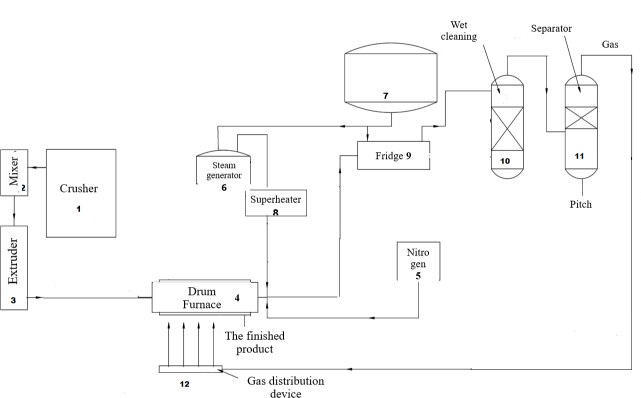
\includegraphics[width=0.8\textwidth]{assets/1004}
	\caption*{Figure 1 -- Technological scheme of the installation for the production of adsorbent}
\end{figure}

\begin{figure}[H]
	\centering
	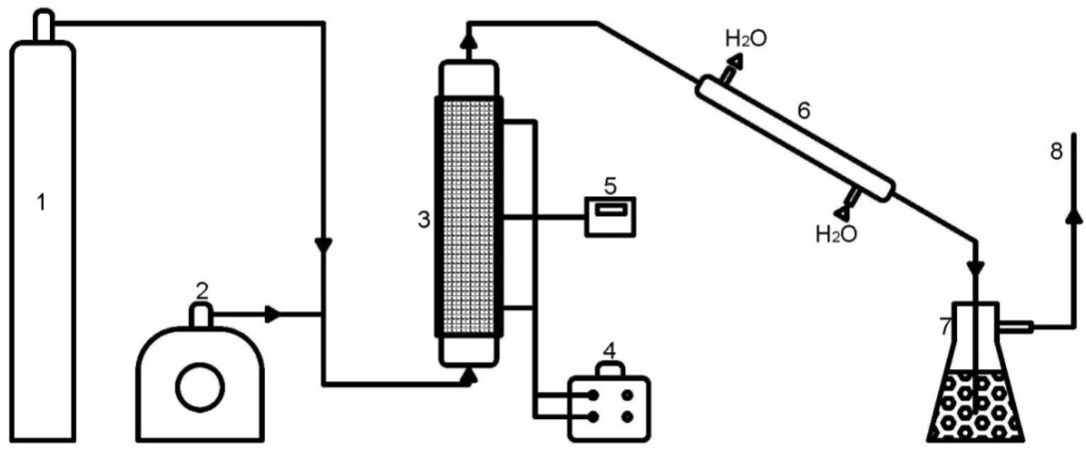
\includegraphics[width=0.5\textwidth]{assets/1005}
	\caption*{Figure 2 -- Schematic diagram of a laboratory installation of steam and gas activation:}
	\caption*{1 -- gas cylinder (argon); 2 -- steam generator; 3 -- reactor; 4 -- LATR; 5 -- thermal sensor; 6 -- direct refrigerator; 7 -- flask for gas purification from resins; 8 -- gas outlet}
\end{figure}

\begin{multicols}{2}
The work is aimed at developing a highly efficient technology and
creating a pilot production of carbon nanoporous materials from waste
materials. Carbon materials can be used to isolate and purify hydrogen
from synthesis gas, release nitrogen from air; purify air from methane,
monoxide and carbon dioxide; clean wastewater from toxic impurities,
manufacture supercapacitors for lithium-ion batteries and catalyst
carriers.

{\bfseries Materials and methods:} The study used methods for obtaining
carbon adsorbents (carbonation and activation) in laboratory conditions,
methods for determining their physico-chemical and adsorption
properties: determination of humidity, ash content, volatility,
pH-aqueous extract, bulk density, adsorption activity by methyl orange,
method for determining the total pore volume by water, elemental
analysis, method BET for determining the specific surface area of the
obtained materials, methods of water purification from oil and iron in
laboratory conditions, methods of wastewater and gas purification from
acidic components, etc.

Instruments were used: laboratory quartz reactor, rotary tubular furnace
BR-12NRT, thermogravimetric analyzer (Thermostep Eltra), Crystallux gas
chromatograph, Shaker Incubator ES-20/60, spectrophotometer (PD-303), pH
meter, centrifuge, ultrasonic bath, muffle furnace, ultrasonic bath,
scanning electron microscopy, X-ray-fluorescent analyzer, energy
dispersion elemental analysis, etc.

{\bfseries Results:} The technological process was carried out in two
stages: carbonation (700°C) (to remove volatile components and obtain a
large-porous structure evenly distributed throughout the volume) and
activation (800°C) (to obtain a microporous structure). The experiments
were carried out on a laboratory installation of steam and gas
activation

A drawing of the laboratory reactor is shown in Figure 2.

Carbonation was carried out in an inert argon medium in the temperature
range of 400-800 C for 60 minutes. Argon was supplied from a cylinder
(1) to a reactor with a predetermined flow rate of 20 ml/min, which was
installed using a flow meter. After the reactor, the gas was sent to the
refrigerator (6), from where part of the condensed gas was poured into
the flask (7) for purification from resinous substances. The unreacted
gases were discharged into the ventilation system (8).

At the next stage of preparation of the adsorbent, to improve its
adsorption properties, activation with water vapor (consumption 10
ml/min) was carried out at a maximum temperature with an exposure time
of 60 minutes.

Table 1 shows the temperature dependences of the components of the gas
obtained as a result of carbonation and activation of the nylon cord.
The formation of combustible gas components (CO, H\textsubscript{2},
CH\textsubscript{4}) occurs in accordance with the basic chemical
reactions:

2H\textsubscript{2}O → 2H\textsubscript{2} + O\textsubscript{2} --
115700 kkal\hfill (1)

C + H\textsubscript{2}O → CO + H\textsubscript{2} -- 28150 kkal\hfill (2)

C + CO\textsubscript{2} → 2CO -- 38400 kkal\hfill (3)

C + 2H\textsubscript{2} → CH\textsubscript{4} + 18600 kkal\hfill (4)

Textile cord under heat treatment above 200°C begins to decompose to
form a combustible gas, which contains hydrogen, carbon monoxide,
alkanes and alkenes.
\end{multicols}

\begin{table}[H]
\caption*{Table 1 -- Gas composition of carbonation and activation of textile cord}
\centering
\resizebox{\columnwidth}{!} \\ \cline{3-11}
 &  & \multicolumn{1}{l|}{О2} & \multicolumn{1}{l|}{H2} & \multicolumn{1}{l|}{CO2} & \multicolumn{1}{l|}{N2} & \multicolumn{1}{l|}{CH4} & \multicolumn{1}{l|}{CO} & \multicolumn{1}{l|}{Ethane} & \multicolumn{1}{l|}{Ethylene} & \multicolumn{1}{p{0.1\textwidth}|}{Propane + Propylene} \\ \hline
\multirow{5}{*}{Carbonation} & 200 & \multicolumn{1}{l|}{37.003} & \multicolumn{1}{l|}{0.046} & \multicolumn{1}{l|}{0.126} & \multicolumn{1}{l|}{32.911} & \multicolumn{1}{l|}{0.166} & \multicolumn{1}{l|}{0.040} & \multicolumn{1}{l|}{0.005} & \multicolumn{1}{l|}{-} & 0.589 \\ \cline{2-11}
 & 300 & \multicolumn{1}{l|}{37.874} & \multicolumn{1}{l|}{0.259} & \multicolumn{1}{l|}{1.139} & \multicolumn{1}{l|}{68.089} & \multicolumn{1}{l|}{0.083} & \multicolumn{1}{l|}{-} & \multicolumn{1}{l|}{0.009} & \multicolumn{1}{l|}{0.335} & 0.020 \\ \cline{2-11}
 & 400 & \multicolumn{1}{l|}{43.355} & \multicolumn{1}{l|}{0.237} & \multicolumn{1}{l|}{2.219} & \multicolumn{1}{l|}{66.944} & \multicolumn{1}{l|}{0.045} & \multicolumn{1}{l|}{-} & \multicolumn{1}{l|}{0.036} & \multicolumn{1}{l|}{0.680} & 0.054 \\ \cline{2-11}
 & 500 & \multicolumn{1}{l|}{34.788} & \multicolumn{1}{l|}{3.380} & \multicolumn{1}{l|}{1.874} & \multicolumn{1}{l|}{58.749} & \multicolumn{1}{l|}{1.082} & \multicolumn{1}{l|}{-} & \multicolumn{1}{l|}{1.095} & \multicolumn{1}{l|}{0.705} & 1.012 \\ \cline{2-11}
 & 600 & \multicolumn{1}{l|}{54.526} & \multicolumn{1}{l|}{10.091} & \multicolumn{1}{l|}{1.671} & \multicolumn{1}{l|}{36.023} & \multicolumn{1}{l|}{2.570} & \multicolumn{1}{l|}{-} & \multicolumn{1}{l|}{0.918} & \multicolumn{1}{l|}{0.565} & 1.012 \\ \hline
\multirow{3}{*}{Activation} & 700 & \multicolumn{1}{l|}{30.469} & \multicolumn{1}{l|}{3.873} & \multicolumn{1}{l|}{0.411} & \multicolumn{1}{l|}{76.123} & \multicolumn{1}{l|}{0.746} & \multicolumn{1}{l|}{-} & \multicolumn{1}{l|}{0.137} & \multicolumn{1}{l|}{0.036} & 0.162 \\ \cline{2-11}
 & 800 & \multicolumn{1}{l|}{28.204} & \multicolumn{1}{l|}{5.608} & \multicolumn{1}{l|}{0.302} & \multicolumn{1}{l|}{75.943} & \multicolumn{1}{l|}{0.813} & \multicolumn{1}{l|}{0.436} & \multicolumn{1}{l|}{0.066} & \multicolumn{1}{l|}{0.080} & 0.082 \\ \cline{2-11}
 & 800 excerpt & \multicolumn{1}{l|}{27.532} & \multicolumn{1}{l|}{3.304} & \multicolumn{1}{l|}{0.157} & \multicolumn{1}{l|}{81.477} & \multicolumn{1}{l|}{-} & \multicolumn{1}{l|}{-} & \multicolumn{1}{l|}{0.038} & \multicolumn{1}{l|}{0.058} & 0.006 \\ \hline
\end{tabular}
}
\end{table}

\begin{table}[H]
\caption*{Table 2 -- Material balance of carbonation and activation of textile cord}
\centering
\begin{tabular}{|lll|l|l|l|}
\hline
\multicolumn{1}{|l|}{№} & \multicolumn{1}{l|}{Incoming products} & Content, \% & № & Outgoing products & Content, \% \\ \hline
\multicolumn{1}{|l|}{1} & \multicolumn{1}{l|}{Textile cord} & 71,49 & 1 & Solid residue (adsorbent) & 22,8 \\ \hline
\multicolumn{1}{|l|}{2} & \multicolumn{1}{l|}{Water (us.steam)} & 28,51 & 2 & Generator gas & 67,22 \\ \hline
\multicolumn{1}{|l|}{} & \multicolumn{1}{l|}{Total} & 100 & 3 & Liquid product (water+resin) & 9,98 \\ \hline
\multicolumn{3}{|l|}{} &  & Total & 100 \\ \hline
\end{tabular}%
\end{table}

\begin{multicols}{2}
The study used methods for obtaining sorbents, methods for determining
ash content, humidity, volatility of raw materials (thermogravimetric
analysis), their physico-chemical and adsorption properties: elemental
analysis; gas chromatography; SEM (scanning electron microscopy), which
determines the total volume, density of sorbents.
\end{multicols}

\begin{figure}[H]
    \centering
    \begin{subfigure}[b]{0.45\textwidth}
        \centering
        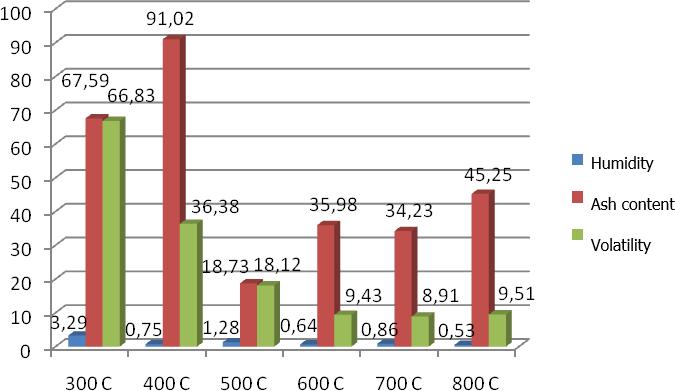
\includegraphics[width=\textwidth]{assets/1006}
        \caption*{Figure 3 -- Results on volatility, ash content and humidity of adsorbents from textile cord}
    \end{subfigure}
    \hfill
    \begin{subfigure}[b]{0.45\textwidth}
        \centering
        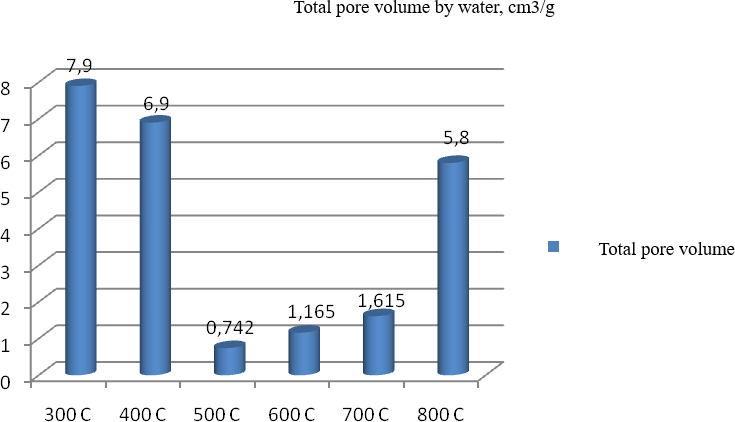
\includegraphics[width=\textwidth]{assets/1007}
        \caption*{Figure 4 -Results of measuring the total pore volume of adsorbents in water at different temperatures}
    \end{subfigure}
\end{figure}

\begin{figure}[H]
	\centering
	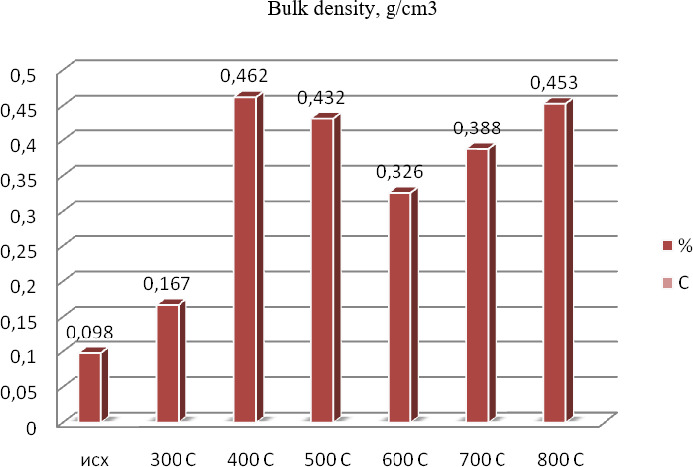
\includegraphics[width=0.6\textwidth]{assets/1008}
	\caption*{Figure 5 -- Bulk density of adsorbents from textile cord}
\end{figure}

\begin{multicols}{2}
Based on the results of determining the total pore volume by water,
porous materials obtained at 300°C, 400°C and 800°C showed the highest
index from 5.8 to 7.9 ml/g. Therefore, this indicates a high degree of
porosity of the adsorbent.

According to the results of determining the density of adsorbents, the
lowest density of adsorbents was shown by the initial product (0.098 g
/cm\textsuperscript{3}), also at 300°C, the value of which was 0.167 g
/cm\textsuperscript{3}. The density of all adsorbents increased compared
to the initial sample.

The study of the elemental composition, structure and dimension of the
samples was carried out by energy dispersive X-ray spectroscopy on a SEM
(Quanta 3D 200i) device with an energy dispersive analysis prefix from
EDAX. The energy of the exciting electron beam in the analysis was 15
keV.

The elemental composition of the initial textile cord is shown in Figure
6.
\end{multicols}

\begin{table}[H]
\centering
\begin{minipage}{0.45\textwidth}
\centering
\begin{tabular}{|l|l|l|}
\hline
Element & Wt\% & At\% \\ \hline
C & 74.10 & 81.40 \\ \hline
O & 20.76 & 17.12 \\ \hline
Na & 0.32 & 0.18 \\ \hline
Al & 0.15 & 0.07 \\ \hline
Si & 0.29 & 0.14 \\ \hline
S & 0.60 & 0.25 \\ \hline
Ca & 0.34 & 0.11 \\ \hline
Fe & 0.90 & 0.21 \\ \hline
Cu & 0.62 & 0.13 \\ \hline
Zn & 1.91 & 0.38 \\ \hline
\end{tabular}%
\end{minipage}\hfill
\begin{minipage}{0.45\textwidth}
\centering
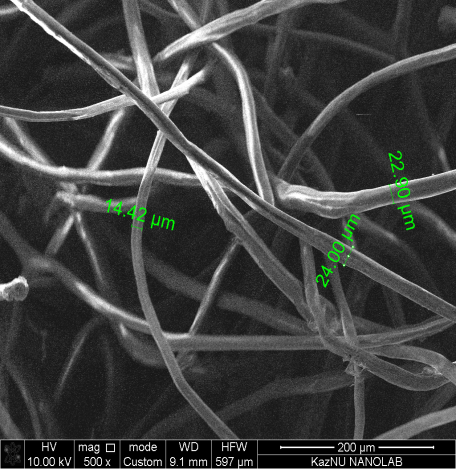
\includegraphics[width=\textwidth]{assets/1009}
\end{minipage}
\caption*{(a)}
\end{table}

\begin{table}[H]
\centering
\begin{minipage}{0.45\textwidth}
\centering
\begin{tabular}{|l|l|l|}
\hline
Element & Wt\% & At\% \\ \hline
C & 89.64 & 93.71 \\ \hline
O & 6.23 & 4.89 \\ \hline
Na & 0.86 & 0.47 \\ \hline
Al & 0.08 & 0.04 \\ \hline
Si & 0.20 & 0.09 \\ \hline
S & 0.29 & 0.13 \\ \hline
Ca & 0.49 & 0.19 \\ \hline
Fe & 0.05 & 0.02 \\ \hline
Cu & 0.30 & 0.09 \\ \hline
Zn & 0.32 & 0.07 \\ \hline
\end{tabular}%
\end{minipage}\hfill
\begin{minipage}{0.45\textwidth}
\centering
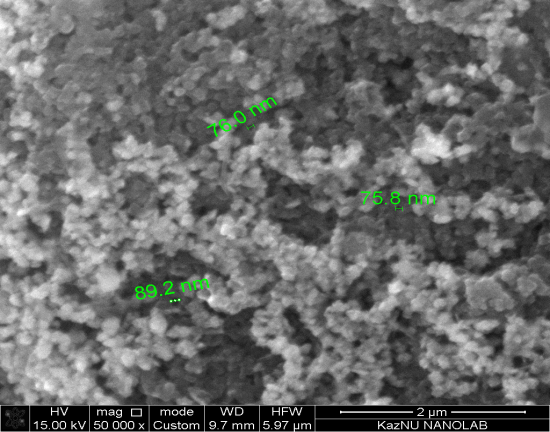
\includegraphics[width=\textwidth]{assets/1010}
\end{minipage}
\caption*{(b)}
\caption*{Figure 6 - SEM images of the original (a) and activated (b) textile cord}
\end{table}

\begin{multicols}{2}
In Figure 6 (a), fiber particles with a diameter of 10 to 25 microns are
clearly visible, the structural elements take the form of fibrils --
filamentous formations.

The results of the analysis of micrographs show (Fig.6 (b)) that after
heat treatment, the surface structure changes with smaller particle
sizes (up to \textasciitilde145 nm), fine carbon nanoparticles with a
diameter from 70 to 600 nm were formed, this may be due to the fact that
as a result of carbonization and activation, the forming
reactively-capable radicals interact with each other to form new
substances. The nucleation and growth of ordered carbon during the heat
treatment of textile cord can occur by self-organization of carbon
nanoparticles without the participation of mesophase, however,
additional research is required to clarify this issue.

In the laboratory of the Institute of Coal Chemistry and Technology LLP,
the obtained carbon nanoporous materials were tested to purify gases
(composition: H\textsubscript{2}S, CO, CO\textsubscript{2},
CH\textsubscript{4}, N\textsubscript{2}, H\textsubscript{2}) from
harmful substances H\textsubscript{2}S, CO\textsubscript{2},
N\textsubscript{2} to obtain mainly combustible components CO,
CH\textsubscript{4}, H\textsubscript{2}. The results of the elemental
analysis before and after gas purifications with determination of the
degree of purification are presented in Table 3.
\end{multicols}

\begin{table}[H]
\caption*{Table 3 -- Approbation of adsorbents from textile cord for gas purification}
\centering
\begin{tabular}{|l|lllll|lllll|}
\hline
\multirow{2}{*}{Name} & \multicolumn{5}{l|}{Gas concentration \%} & \multicolumn{5}{l|}{Degree of purification, \%} \\ \cline{2-11}
 & \multicolumn{1}{l|}{H2} & \multicolumn{1}{l|}{CO2} & \multicolumn{1}{l|}{CH4} & \multicolumn{1}{l|}{CO} & H2S & \multicolumn{1}{l|}{H2} & \multicolumn{1}{l|}{CO2} & \multicolumn{1}{l|}{CH4} & \multicolumn{1}{l|}{CO} & H2S \\ \hline
Crude source gas & \multicolumn{1}{l|}{46,817} & \multicolumn{1}{l|}{2,091} & \multicolumn{1}{l|}{7,05} & \multicolumn{1}{l|}{7,546} & 0,045 & \multicolumn{1}{l|}{-} & \multicolumn{1}{l|}{-} & \multicolumn{1}{l|}{-} & \multicolumn{1}{l|}{-} & - \\ \hline
Activated Textile cord & \multicolumn{1}{l|}{0,165} & \multicolumn{1}{l|}{0,075} & \multicolumn{1}{l|}{0,151} & \multicolumn{1}{l|}{0,047} & 0,007 & \multicolumn{1}{l|}{99,6} & \multicolumn{1}{l|}{96,4} & \multicolumn{1}{l|}{97,8} & \multicolumn{1}{l|}{99,3} & 84,4 \\ \hline
\end{tabular}
\end{table}

\begin{multicols}{2}
{\bfseries Conclusion:} Known methods of cleaning natural objects are not
always effective, and are often environmentally unsafe. The use of
organic waste for wastewater and atmospheric treatment is acceptable
from an economic and environmental point of view, but as a rule, such
materials do not have sufficiently capacious sorption properties and
therefore they need to be carbonized and activated. As a result,
sorbents with a surface different from the original mineral are obtained
and combine the useful characteristics of the starting material and
synthetic sorbents.

In the course of the work done, a laboratory installation for the
production of adsorbents was assembled, work was carried out to improve
the methodology and technology for the production of nanosorbents, with
the determination of optimal technological parameters. The
physicochemical properties of the feedstock and the obtained adsorbents
(ash content, humidity, volatility, bulk density, total pore volume,
elemental composition) were also studied. The resulting product has been
tested for gas purification. The degree of gas purification (\%) was
H\textsubscript{2}-99.6; CO\textsubscript{2}-96.4;
CH\textsubscript{4}-97.8; CO-99.3; H\textsubscript{2}S-84.4.

\emph{{\bfseries Financing}.The research was carried out with the financial
support of the Science Committee of the Ministry of Science and Higher
Education of the Republic of Kazakhstan (Grant No. AR19577512.
Development of scientific and technical foundations for the production
of microporous carbon nanomaterials for the separation and storage of
hydrogen).}
\end{multicols}

\begin{center}
{\bfseries References}
\end{center}

\begin{noparindent}
1. Rezoljucija Vserossijskoj konferencii "Novaja gosudarstvennaja
jekologicheskaja politika v real\textquotesingle nom sektore
jekonomiki", 22.11.2005, Moskva, Kreml\textquotesingle{} (in Russian)

2. Tehnologija pererabotki tverdogo ostatka piroliza avtoshin v
formovannoe toplivo / Papin A.V., Ignatova A.Ju., Nevedrov A.V.,
Shikanova K.A // Polzunovskij vestnik 2015, № 2. S. 106-108. (in
Russian)

3. Shapranko D.S., Bazanov M.M. Jekologicheski bezopasnye
resursosberegajushhie tehnologii pererabotki

rezinotehnicheskih izdelij,
primenjaemye v Kuzbasse / Materialy II regional\textquotesingle noj
nauchno-prakticheskoj

konferencii studentov i
shkol\textquotesingle nikov «Jekologija Kuzbassa». Kemerova: KuzGTU,
2015. (in Russian)

4. Novichkov Ju. A., Petrenko T.V., Bratchun V.I. Issledovanie processa
beskislorodnogo piroliza iznoshennyh avtomobil\textquotesingle nyh shin
// Vestnik Har\textquotesingle kovskogo nacional\textquotesingle nogo
avtomobil\textquotesingle no-dorozhnogo universiteta. 2005. № 29. S.
68-70. (in Russian)

5. Frolov Ju.N. Organizacija zashhity okruzhajushhej prirodnoj sredy v
avtotransportnom komplekse // Avtomatiz. i sovrem, tehnol. -- 1997. -
№7. -- S.37-44. (in Russian)

6. Tarasevich M.R. Jelektrohimija uglerodnyh materialov. M.: Nauka,
1984. -253 s.

7. Drugov Ju.S., Rodin A.A. Jekologicheskie analizy pri razlivah nefti i
nefteproduktov.-M.: BINOM. Laboratorija znanij, 2010.- S. 6-20. (in
Russian)

8. Farmakovskij B.V., Dzhurinskij D.V.//Issledovanija processa
nanesenija pokrytij iz raznorodnyh materialov na metallicheskie
podlozhki metodom HGDN. Voprosy materialovedenija. 2003. №2 (34). (in
Russian)

9. Muhutdinov A.A., Minhajdarova G.V., Muhutdinov Je.A. Primenenie
tverdogo ostatka piroliza dlja ochistki stochnyh vod // Jekologija i
promyshlennost\textquotesingle{} Rossii. 2006 №7. S.37-41. (in Russian)

10. Vajnerman A.E., Kirilin Je.F., Rybin V.V., Chumakova I.V., Shekalov
B.I.//Problemy i dostizhenija v oblasti sozdanija mednyh splavov,
prisadochnyh materialov i tehnologii svarki i naplavki dlja izdelij
sudovogo

mashinostroenija. Voprosy materialovedenija, 1999. №3 (20)-S.
241-260. (in Russian)
\end{noparindent}
\newpage
\emph{{\bfseries Information about the authors}}

\begin{noparindent}
Kazankapova M.K. {\bfseries -} PhD in Philosophy, assoc. professor, member
correspondent of the KazNANS, Project Manager, Leading Researcher, Head
of Laboratory of LLP "Institute of Coal Chemistry and Technology",
Astana, Kazakhstan, e-mail: maira\_1986@mail.ru;

Yermagambet B.T. - Doctor of Chemical Science, Professor, Academician of
the KazNANS, Chief Researcher, Director of LLP "Institute of Coal
Chemistry and Technology", Astana, Kazakhstan, e-mail: bake.yer@mail.ru;

Kozhamuratova U.M. {\bfseries --} master student Eurasian National
University of L.N. Gumilyov{\bfseries ,} Astana, Kazakhstan, e-mail:
kozhamuratova.u@mail.ru;

Malgazhdarova A.B. {\bfseries --} master student Eurasian National
University of L.N. Gumilyov{\bfseries ,} Astana, Kazakhstan, e-mail:
malgazhdarova.ab@mail.ru.
\end{noparindent}

\emph{{\bfseries Сведения об авторах}}

\begin{noparindent}
Казанкапова М.К.- PhD философских наук, асс. профессор, чл.-корр.
КазНАЕН, руководитель проекта, ведущий научный сотрудник, заведующая
лабораторией ТОО «Институт химии и технологии угля», Астана, Казахстан,
e-mail: maira\_1986@mail.ru;

Ермагамбет Б.Т. -доктор химических наук, профессор, академик КазНАЕН,
главный научный сотрудник, директор ТОО «Институт химии и технологии
угля», Астана, Казахстан, e-mail: bake.yer@mail.ru;

Кожамуратова У.М. -- магистрант Евразийского национального университета
им. Л.Н. Гумилева, Астана, Казахстан, e-mail: kozhamuratova.u@mail.ru;

Малгаждарова А.Б. -- магистрант Евразийского национального университета
им. Л.Н. Гумилева, Астана, Казахстан, e-mail: malgazhdarova.ab@mail.ru.
\end{noparindent}
